\documentclass[11pt, oneside]{article}
\usepackage[margin=1in]{geometry}
\geometry{letterpaper}
\usepackage{booktabs}
\usepackage{hyperref}
\usepackage{enumitem}
\usepackage{float}
\usepackage{caption}
\usepackage{subcaption}
\usepackage[numbers]{natbib}
\usepackage{graphicx}
\usepackage{amssymb}
\usepackage{amsmath}
\usepackage{array}
\usepackage{longtable}
\usepackage{xcolor}
\usepackage{tabularx}
\usepackage{setspace}
\usepackage{tikz}
\usetikzlibrary{positioning,arrows.meta,fit}
\usepackage{pgfplots}
\usepackage{adjustbox}
\pgfplotsset{compat=1.17}
\hypersetup{
    colorlinks=true,
    linkcolor=blue,
    citecolor=blue,
    urlcolor=blue
}
% ------------------------------------------------------------------
% DRAFT MARKER: every \todo{...} must be replaced by the student's own
% text (or removed) before submission.  grep -n 'todo{' to find them.
% ------------------------------------------------------------------
\newcommand{\todo}[1]{\textcolor{red}{\textbf{[TODO (student): #1]}}}
\newcommand{\tbd}{\textcolor{red}{\textbf{??}}}
\newcommand{\tsc}[1]{\texttt{\detokenize{#1}}}
\captionsetup{font=small,skip=3pt}
\setlength{\textfloatsep}{8pt plus 2pt minus 2pt}
\setlength{\floatsep}{6pt plus 2pt minus 2pt}
\setlength{\intextsep}{6pt plus 2pt minus 2pt}
% ============================================================
% TITLE BLOCK --- students must keep this format
% ============================================================
\title{CS781 Capstone Project:\\
In-House Legal Intelligence System}
\author{
    Dhruv Shetty \todo{full name as on records, middle name if any}  \\
    230370 \\
    {\tt \todo{userid}@iitk.ac.in}\\
    Indian Institute of Technology Kanpur (IIT Kanpur)
}
\date{}
\begin{document}
\maketitle
\begin{abstract}
A law firm needs a confidential legal NLP stack that runs without external LLM APIs or third-party pretrained weights. We pretrained four 100--125M-parameter models from scratch on 0.97B tokens of Indian court and statute text with our own 32k BPE tokenizer (decoder-only, encoder--decoder, prefix-LM and sliding-window/GQA) and adapted them to legal NER, rhetorical roles, judgment prediction, statute identification, summarization and prior-case retrieval with self-implemented parameter-efficient methods and distillation into half-depth students. Backbones with bidirectional context (prefix-LM, BART encoder) gave the best official score in four of the five understanding tasks, and LoRMA, training 0.2--0.4\% of the parameters, produced the best submission in Phases~3--7 and came within 0.04 of full fine-tuning in Phase~2. The largest remaining losses come from decision rules rather than representations: a fixed 0.5 threshold halves statute-identification macro-F1 relative to a dev-fitted one, and greedy summaries repeat themselves.
\end{abstract}

\noindent\textbf{Code:} \url{https://github.com/DhruvShetty22/cs781-legal-nlp-capstone} \todo{confirm the final repository URL after pushing}

% ============================================================
\section{Competition Result}
% ============================================================
\noindent
\textbf{Codabench username:} d\_230370 \todo{confirm}
\hfill
\textbf{Roll number:} 230370
\begin{table}[H]
\centering
\caption{Official phase scores and ranks.}
\label{tab:leaderboard}
\begin{tabular}{clccc}
\toprule
Phase & Task & Primary metric (value) & Rank & Valid submissions \\
\midrule
1 & Legal LM Pretraining & BERTScore F1 = 0.8294$^{*}$ & \tbd & 5$^{*}$ \\
2 & Legal NER & Strict Macro-F1 = 0.4399$^{*}$ & \tbd & 5 \\
3 & Rhetorical role prediction & Macro-F1 = 0.4373$^{*}$ & \tbd & 7 (5 distinct)$^{*}$ \\
4 & Court judgment prediction & Macro-F1 = 0.6371$^{*}$ & \tbd & 5$^{*}$ \\
5 & Legal statute identification & Macro-F1 = 0.1651$^{*}$ & \tbd & 3$^{*}$ \\
6 & Abstractive summarization & BERTScore F1 = 0.7662$^{*}$ & \tbd & 6 \\
7 & Prior Case Retrieval (PCR) & Micro-F1@7 = 0.3166 & \tbd & 5 \\
\bottomrule
\end{tabular}
\end{table}
\noindent{\footnotesize $^{*}$Phase~1 includes the course's starter-code output (not counted towards the minimum); Phase~3 counts 7 finished uploads of 5 distinct files; in Phase~5, 1 upload failed and 2 were never evaluated. The highest Phase-6 score, 0.7686 (\tsc{llama} LoRMA), is not the leaderboard entry. Submission IDs and how each was matched to its run are in Appendix~\ref{app:p1attr}; three Phase-1/2 matches and one Phase-5 match are inferred. \todo{confirm the inferred matches}}

\noindent
\textbf{Total valid Codabench submissions across all phases:} 36 finished (33 distinct, excluding the starter-code output)
\quad
\textbf{Date ranks were recorded:} \tbd
\smallskip

\noindent Counting finished, distinct submissions, the minimum of four is met in every phase except Phase~5. There, one of six uploads failed and two were never evaluated by Codabench, which left three scored submissions.

% ============================================================
\section{Introduction and Problem Description}
% ============================================================
The firm's brief is to automate routine legal-document work on Indian case law without sending privileged documents to an external service. This rules out commercial LLM APIs and models pretrained by third parties. Every model we use therefore descends from language models we pretrained ourselves on the provided corpus, and every later capability is obtained by adapting those models. The seven tasks follow the IL-TUR benchmark~\cite{joshi2024iltur}; Table~\ref{tab:tasks} gives the input, output and metric of each.

\begin{table}[t]
\centering
\small
\caption{Task definitions (capstone \S7--\S13). All data comes from \tsc{Exploration-Lab/CS-781-Capstone}.}
\label{tab:tasks}
\begin{tabularx}{\textwidth}{c l X l}
\toprule
Ph. & Task & Input $\rightarrow$ output (\tsc{prediction.json}) & Primary metric \\
\midrule
1 & LM pretraining & 512-word judgment prompt $\rightarrow$ 128-word continuation & BERTScore F1 \\
2 & L-NER & judgment text $\rightarrow$ list of \tsc{[start, end, label]} character spans, 12 labels & strict Macro-F1 \\
3 & Rhetorical roles & list of sentences $\rightarrow$ one of 13 roles per sentence (CL and IT subsets) & Macro-F1 \\
4 & CJPE & full judgment $\rightarrow$ outcome $\in\{0,1\}$ & Macro-F1 \\
5 & Statute ID & case facts $\rightarrow$ set of statute IDs (multi-label) & Macro-F1 \\
6 & Summarization & full judgment $\rightarrow$ abstractive summary & BERTScore F1 \\
7 & Prior-case retrieval & query case + split-specific candidate pool $\rightarrow$ top-7 candidate IDs & Micro-F1@7 \\
\bottomrule
\end{tabularx}
\end{table}

Several constraints shaped the design. The Phase-1 model must have 50M--300M parameters and be trained from random initialisation on the provided corpus. Training ran on free Colab T4 GPUs (16\,GB) whose sessions can be killed, so every run checkpoints to a private Hugging Face repository and every Phase-2--7 run has a hard 60-minute training cap. Phase~2 is scored by strict character-offset span matching, so the token offsets must invert exactly. Phase~5 is multi-label over 100 statutes. Phases~1 and~6 are scored with BERTScore~\cite{zhang2020bertscore}, with ROUGE~\cite{lin2004rouge} and BLEU~\cite{papineni2002bleu} as secondary metrics. Phases~4--7 have documents far longer than our 1024-token context.

We investigated five questions: (i)~which architecture family to pretrain (decoder-only, encoder--decoder, prefix-LM or sliding-window/GQA), and how each transfers; (ii)~how parameter-efficient methods, with LoRMA~\cite{bihany2025lorma} compulsory, compare with each other and with full fine-tuning on a small from-scratch backbone; (iii)~whether distillation into a half-depth student preserves quality; (iv)~how to encode long documents under a 512-token chunk budget; and (v)~phase-specific choices, namely NER tagging and decoding, sentence context, multi-label thresholds, generation decoding, and ranking losses and negatives.
\textbf{Scope.} Every phase is built end to end in one notebook template, which is rendered into four per-architecture notebooks. Each covers data loading, preprocessing, model, training, local evaluation with the official scorer, and submission packaging. All PEFT and KD code is our own PyTorch~\cite{paszke2019pytorch}; we did not use \tsc{peft} or \tsc{bitsandbytes}. Backbones are Transformers~\cite{wolf2020transformers} classes built from our own configs and weights. We did not attempt prefix tuning, external or synthetic data, cross-encoder re-ranking, or chaining phases together; each phase fine-tunes its own copy of a Phase-1 model.

% ============================================================
\section{Data Analysis and Preprocessing}\label{sec:data}
% ============================================================
\subsection{Sources and official splits}
We used only the official \tsc{Exploration-Lab/CS-781-Capstone} dataset and its phase configurations. Table~\ref{tab:splits} (Appendix~\ref{app:extra}) lists the sizes reported by our data-loading code.

\subsection{Corpus statistics that informed design}
\textbf{Phase 1.} After sampling, the training token counts per source are 252.5M (Supreme Court), 396.6M (High Courts), 250.3M (tribunals) and 75.0M (Acts) (Fig.~\ref{fig:data}a, Appendix~\ref{app:extra}). The tokenizer averages 1.213 tokens per word on the held-out references. During training, sources are drawn with probabilities 0.35/0.35/0.15/0.15 (SC/HC/tribunal/Acts) rather than in proportion to their size. Relative to their share of tokens (26\%, 41\%, 26\% and 8\%), this up-weights the Supreme Court and the statutes and down-weights the High Courts and tribunals, so that no single source dominates the windows the model sees.
\textbf{Phase 2.} The 70 labelled documents contain 8393 spans, ranging from 184 for R.COUNSEL to 1575 for DATE (Fig.~\ref{fig:data}b). All spans satisfy \tsc{text[s:e]} (end-exclusive), with no invalid or overlapping spans. Documents have a median of 26,620 characters (5533 tokens).
\textbf{Phase 3.} The training sets have 10,593 CL and 6252 IT sentences. The two dominant roles are Fact (2979 CL / 1119 IT) and RatioOfTheDecision (2856 / 1445). Dissent (284 CL train sentences) and PrecedentOverruled (3 IT train sentences) do not occur in dev, which caps the attainable dev macro-F1 at 0.8462. 1.9\% of sentences exceed the 128-token sentence cap.
\textbf{Phase 4.} The raw train file has 37,387 records. 5082 of them repeat an ID (none with a conflicting label) and are dropped, leaving 32,305 documents (18,920 label 0 / 13,385 label 1). Dev is balanced (497/497). At 512 tokens per chunk and 8 chunks, 28.9\% of train and 45.5\% of dev documents are longer than the budget, and 62--63\% of tokens are seen at prediction time.
\textbf{Phase 5.} There are 100 statute IDs, and each has at least 200 training documents. Documents carry 3.70 statutes on average in train (max 31) and 3.92 in dev. The three most frequent IDs cover 27.4\%, 24.3\% and 18.4\% of training documents, and the label sets are diverse (16,191 distinct sets). Predicting the most frequent statute for every document gives a dev macro-F1 of 0.0045.
\textbf{Phase 6.} Documents have a median of 3129 words and summaries a median of 638 words. 99.5\% of documents exceed 512 tokens and 76.6\% of summaries exceed 480 tokens. On our held-out set, the whole document covers 95.3\% of reference unigrams and the first 512 tokens cover 39.7\% (53.6\% at 768 tokens).
\textbf{Phase 7.} Queries have 6.42 relevant candidates on average in train (max 52; 10 queries have none) and 8.25 in dev (max 92). Each split has its own pool. 55--67\% of documents exceed the 8-chunk budget. On dev, the oracle top-7 reaches F1@7 0.6181 and random ranking 0.0074; our word-level BM25 scores 0.1123.

\subsection{Preprocessing}
\textbf{Tokenization.} All phases use the Phase-1 32k byte-level BPE tokenizer on cased text with the original punctuation and Unicode. No special tokens are inserted, and token IDs are cached as \tsc{uint16}.
\textbf{Phase-2 offsets.} Each document is tokenized once with \tsc{return_offsets_mapping}. Token character ranges are trimmed of whitespace, and whitespace-only tokens get empty ranges. A token takes its B-/I- tag (BIO, 25 tags) from the gold span covering its first visible character. When decoding, whitespace tokens are transparent, and a span runs from the first to the last visible character of its tokens. Round-tripping the gold spans through this encoding gives a strict macro-F1 of 0.9863, which is the ceiling our encoding allows. We use 512-token windows with stride 256 for training and 128 for prediction, and overlapping predictions are averaged per token.
\textbf{Phase-3 sentences.} The provided sentence lists are kept unchanged. Each sentence is encoded as \tsc{" " + s.strip()} (at most 128 tokens), and predictions are written back by index, so output length always equals input length. Whole sentences are packed into windows of at most 512 tokens and 24 sentences. Windows use stride 12 for training and 6 for prediction, with scores averaged over windows.
\textbf{Long documents.} In Phases~4, 5 and~7, the whole document is cut into 512-token chunks, plus a final chunk that ends at the document end. \tsc{CHUNK_SELECT=even} keeps at most 8 evenly spaced chunks; Phase~7 keeps 4 during training. Phase~6 instead truncates the source to its head (512 tokens; 768 for BART) and caps the summary at 480 (512) tokens.
\textbf{Phase~7} queries and candidates share one encoder and the same chunking. A query's own ID is excluded from its ranking, and positives are the relevant candidates found in the training pool (5308 pairs from 817 queries).

% ============================================================
\section{Approach and Model Evolution}
% ============================================================
\subsection{Phase-1 foundation model}\label{sec:p1}
We pretrained four architecture families from random initialisation (Table~\ref{tab:p1arch}). All are Hugging Face model classes built from our own configs, with tied input/output embeddings and $d_\text{model}=768$. The parameter count is printed by the training notebook (\tsc{sum(p.numel())}), and all four are inside the 50M--300M bound.

\begin{table}[t]
\centering
\footnotesize\setlength{\tabcolsep}{4pt}
\caption{Phase-1 architectures (all $d_\text{model}{=}768$, vocabulary 32k, tied embeddings).}
\label{tab:p1arch}
\begin{adjustbox}{max width=\textwidth}\begin{tabular}{l c c c c}
\toprule
& \tsc{llama} & \tsc{prefixlm} & \tsc{mistral_swa} & \tsc{bart} (v2) \\
\midrule
Family & decoder-only & prefix-LM hybrid & efficient (SWA+GQA) & encoder--decoder \\
Layers & 12 & 12 & 12 & 6 enc + 6 dec \\
Heads (query / KV) & 12 / 12 & 12 / 12 & 12 / 4 & 12 / 12 \\
FFN & SwiGLU 2048 & SwiGLU 2048 & SwiGLU 2048 & GELU 3072 \\
Norm / positions & RMSNorm / RoPE & RMSNorm / RoPE & RMSNorm / RoPE & post-LN / learned \\
Attention & causal & bidir.\ prefix + causal & causal, window 256 & bidir.\ enc, causal dec \\
Context & 1024 & 1024 & 1024 & enc $\le$768, dec 256 \\
Objective & next token & next token after prefix & next token & continuation + infilling \\
Parameters & 109,529,856 & 109,529,856 & 100,092,672 & 125,442,048 \\
\bottomrule
\end{tabular}\end{adjustbox}
\end{table}

\textbf{Tokenizer and data.} The tokenizer is a 32k byte-level BPE~\cite{sennrich2016bpe} trained on 0.4B characters of the corpus (min.\ frequency 2). Each source is tokenized into its own binary file with an end-of-text token after every document. A training window is built by drawing a source with the mixing probabilities above and then taking a random contiguous window. \textbf{Objectives.} \tsc{llama}~\cite{touvron2023llama} and \tsc{mistral_swa}~\cite{jiang2023mistral,ainslie2023gqa} use next-token cross-entropy on all 1024 positions. \tsc{prefixlm}~\cite{raffel2020t5} draws a prefix length $P\sim\mathcal{U}[64,896)$, attends bidirectionally inside the prefix and computes the loss only on tokens after it. BART~\cite{lewis2020bart} v1 encodes the last $S\sim\mathcal{U}[128,768]$ tokens of a window and decodes the next 256. \textbf{Training.} All runs used AdamW~\cite{loshchilov2019adamw} ($\beta=(0.9,0.95)$, weight decay 0.1), peak LR $6\times10^{-4}$ with 300 warm-up steps and cosine decay to $6\times10^{-5}$, 64 windows per step, fp16 autocast and a 3-hour budget. The checkpoint with the lowest validation loss (averaged over the 4 sources) is kept. Tokens seen were 143.9M (llama), 130.7M (prefixlm) and 228.7M (BART-v2); the mistral\_swa run log was not kept. \textbf{Decoding.} At submission time we decode greedily with the prompt truncated to its last 800 tokens (768 for BART). We generate exactly 224 new tokens and cut the output to 128 words. Two configurations were compared on the held-out set: repetition penalty 1.2 and \tsc{no_repeat_ngram_size=4}.

\textbf{What failed first.} The first BART run (v1) collapsed: its decoder ignored the encoder and produced the same continuation for every prompt. We diagnosed this with a probe that compares outputs and losses across prompts (\tsc{bart_diagnostic_cell.py}). We then retrained BART as v2 in a fresh repository with two changes. First, each micro-batch is, with probability 0.5, BART text infilling: Poisson(3) spans covering 30\% of a 512-token window, each replaced by one \tsc{<mask>}, which the decoder rebuilds. Second, a \tsc{<mask>} token is appended to continuation prompts. Wiring checks run at the start of training. At the end of training, the v2 monitor printed a continuation loss of 2.8543 with the model's own prompt versus 3.5813 with another document's prompt, and 8 distinct greedy outputs out of 8. The fix came after the Phase-1 and Phase-2 deadlines (6 and 11~Oct.); v2 was retrained on 14--15~Oct. The Phase-1 leaderboard therefore never saw a working BART: its only BART entry is v1, whose 1000 test continuations are one identical 128-word text. Phase-2 BART runs could only fine-tune the v1 checkpoint. The v2 Phase-1 score (0.8260) is a local held-out number only. Phases~3--7 load BART from v2. An earlier single-notebook pipeline (\tsc{initial_pipeline/}) used a 0.40/0.30/0.20/0.10 mix and a 5.5-hour budget. It was replaced by the per-architecture template before the logged runs.

\subsection{Transfer protocol (Phases 2--7)}
Every Phase-2--7 model is initialised from a Phase-1 \tsc{best/} checkpoint. We do not train any task model from scratch. Each phase has one percent-format template whose configuration cell selects the architecture, the adaptation method and the task-specific options. A builder renders the template into four notebooks, which ran in parallel on four Colab accounts (Fig.~\ref{fig:system}, Appendix~\ref{app:extra}). Decoder backbones (\tsc{llama}, \tsc{prefixlm}, \tsc{mistral_swa}) keep their Phase-1 attention pattern by default. For BART, Phases~2--5 and~7 use the encoder (optionally encoder+decoder), and Phase~6 uses the full model. Table~\ref{tab:methods} (Appendix~\ref{app:extra}) lists the methods implemented and submitted in each phase. LoRA~\cite{hu2021lora} adds $\tfrac{\alpha}{r}BAx$ to $W_0x$, and rsLoRA~\cite{kalajdzievski2023rslora} rescales by $\alpha/\sqrt{r}$. LoRMA~\cite{bihany2025lorma} is multiplicative, $h=(I+\tfrac{\alpha}{r}BA)W_0x$ (\tsc{plus}; a permutation-based rank-inflated variant \tsc{pi} is also implemented), with $B=0$ at initialisation. We verified this with an ``output change at init $=0$'' check, and the adapters are merged into $W_0$ after training (merge checks print logit changes $\le 10^{-4}$). QLoRA~\cite{dettmers2023qlora} uses our own NF4 quantisation with double quantisation. AdaLoRA~\cite{zhang2023adalora} uses an SVD-form update with importance-based rank allocation. Adapters follow Houlsby~\cite{houlsby2019adapters} and Pfeiffer~\cite{pfeiffer2021adapterfusion}. IA$^3$~\cite{liu2022ia3} rescales key, value and FFN activations, prompt tuning~\cite{lester2021prompt} prepends 20 soft tokens, and BitFit~\cite{benzaken2022bitfit} trains only biases and norms. KD~\cite{hinton2015kd} trains a student of the same family that keeps every second Phase-1 block (BART encoder: blocks 0, 2, 4) on
\begin{equation}
\mathcal{L}_\text{KD}=\tfrac12\,\mathcal{L}_\text{task}+\tfrac12\,T^2\,\mathrm{KL}\!\left(\sigma(z_t/T)\,\|\,\sigma(z_s/T)\right),\quad T=2,
\end{equation}
using the teacher run's saved training-set scores. Phase~5 uses a sigmoid/BCE version of this loss and Phase~6 uses sequence-level KD on teacher-generated summaries. LoRMA at rank 8 trained 0.15--0.44M parameters (0.2--0.4\% of the backbone), and every LoRMA run fitted the 60-minute cap with at most 3.6\,GB of GPU memory (Appendix~\ref{app:runs}). In Phase~6, prompt tuning with 15.4K parameters came within 0.003 BERTScore of LoRMA on Codabench for both \tsc{llama} and BART. In Phase~2, full fine-tuning of \tsc{llama} (0.4399) scored above LoRMA with a CRF head (0.4038), but that comparison changes the method and the head at once. Distillation was nearly free in Phases~3 and~4: the BART student is within 0.007 of BART LoRMA on Codabench and, in Phase~4, above its \tsc{llama} teacher, after 10.6 instead of 60 training minutes and with 5$\times$ faster dev inference. In Phase~5, where the student must reproduce 100 sigmoid outputs, it lost 0.049 dev macro-F1.

\subsection{Phase 2 - Legal NER}
We use token classification and reconstruct character offsets from it (\S\ref{sec:data}). The head is dropout 0.1 followed by a linear layer to 25 BIO tags, optionally followed by our own linear-chain CRF~\cite{lafferty2001crf} with Viterbi decoding over the whole document. Window-level scores (softmax probabilities, or CRF emissions) are averaged per token before decoding. The O-tag loss weight was 1.0. Decoding is \emph{lenient} (an I-X tag may open a span) or \emph{strict} (only B-X opens one). Submitted variants include full fine-tuning of three architectures and LoRMA with a CRF head on \tsc{llama}. Only the collapsed BART v1 checkpoint existed during Phase~2 (\S\ref{sec:p1}), so any Phase-2 BART run fine-tuned v1. A BART run on the collapsed v1 checkpoint produced 39,953 test spans, 7--12 times as many as the other runs and some thousands of characters long, consistent with v1's encoder states being unusable for tagging.

\subsection{Phase 3 - Rhetorical role prediction}
Each sentence's vector is the mean of its token states inside a multi-sentence window (\S\ref{sec:data}). The window gives every sentence left context and, for bidirectional backbones (prefixlm, BART encoder), right context as well. A linear layer maps sentence vectors to the 13 roles. CL and IT are trained jointly, and model selection uses macro-F1 on the pooled dev set.

\subsection{Phase 4 - Court judgment prediction}
The model is hierarchical. Each selected 512-token chunk is encoded independently, a chunk vector is the mean of its token states, and a document vector pools the chunk vectors (\tsc{mean}). The head is dropout 0.1 followed by a 2-way linear layer trained with cross-entropy. Prediction uses argmax (threshold 0.5).

\subsection{Phase 5 - Legal statute identification}
This phase uses the same hierarchical encoder as Phase~4, with 100 independent sigmoid outputs trained with binary cross-entropy. The submitted decision rule is a global threshold of 0.5. For reference, the notebook also fits a global threshold and per-label thresholds on dev; because those are fitted on the evaluation data, we report them only as diagnostics (Appendix~\ref{app:runs}).

\subsection{Phase 6 - Abstractive summarization}
Decoder-only backbones see the document, then the separator \texttt{"\textbackslash n\textbackslash nSummary:\textbackslash n"}, then the summary and EOS, with the loss on summary tokens only. The prefix-LM attends bidirectionally over the document, and its generation path is patched so that the prefill is bidirectional too. BART encodes \tsc{document + <mask>} and decodes the summary. We use one truncated pass over the document head rather than chunk-and-merge. Decoding is greedy with \tsc{max_new_tokens} 480 (512 for BART), no $n$-gram blocking and repetition penalty 1.0. No post-training or alignment step was used. The held-out set is 300 training documents (seed 42), and checkpoints are selected by held-out loss.

\subsection{Phase 7 - Prior Case Retrieval (PCR)}
We use a shared-weight bi-encoder: chunk vectors are mean-pooled token states, and the document vector is the mean over chunks. Relevance is $s(q,d)=\cos(\mathbf{q},\mathbf{d})/\tau$ with $\tau=0.05$. The default loss is InfoNCE~\cite{oord2018cpc},
\begin{equation}
\mathcal{L}=-\log\frac{e^{s(q,d^+)}}{e^{s(q,d^+)}+\sum_{d\in\mathcal{N}(q)}e^{s(q,d)}},
\end{equation}
over in-batch candidates plus one random hard negative per pair, with the query's other positives masked out. The alternative loss is ListNet~\cite{cao2007listnet} with a uniform target over the relevant candidates. Long documents are handled by the chunk budget of \S\ref{sec:data}. At test time we embed the split's pool once, score each query against it, drop the query's own ID and output the top~7. A word-level Okapi BM25~\cite{robertson2009bm25} ($k_1{=}1.2$, $b{=}0.75$) is built in as a reference and as a negative miner; BM25 fusion and re-ranking exist but were off in the submitted runs. Word-level BM25 reached only 0.1123 dev F1@7, below the Phase-1 encoders used without any Phase-7 training (0.24--0.26), so BM25 fusion was left off.

% ============================================================
\section{Experiments and Implementation Details}
% ============================================================
\subsection{Compute and training protocol}
All runs used free Colab Tesla T4 GPUs with PyTorch 2.11 and Transformers 5.18, with four accounts running the four architectures in parallel. Each run writes its configuration, metrics, predictions and (merged) model to \tsc{runs/<RUN_NAME>/} in a private Hugging Face repository. Phase~1 additionally saves a \tsc{latest/} checkpoint every 30 minutes and resumes from it after a disconnect. Phases~2--7 share one recipe: AdamW with weight decay 0.01, a head learning rate of $10^{-3}$, 6\% linear warm-up followed by linear decay, gradient clipping at 1.0, fp16 autocast, seed 42, and a 60-minute training cap. Phases~2--3 evaluate after every epoch, and Phases~4--7 evaluate every 10--12 training minutes. The checkpoint with the best dev metric is kept, and training stops after 3 evaluations without improvement (Phase~6 selects by held-out loss). Wall-clock times per run are in Appendix~\ref{app:runs}.

\begin{table}[t]
\centering
\footnotesize
\caption{Hyperparameters of the best-scoring Codabench submission per phase ($^\dagger$ inferred, App.~\ref{app:p1attr}). Parameters: trainable / total for adapted runs. LoRMA is \tsc{plus}, $r{=}8$, $\alpha{=}16$ on \tsc{q_proj}/\tsc{v_proj}. Context: P1 1024-token windows; P2 512-token windows; P3 up to 24 sentences / 512 tokens; P4, P5 8 chunks of 512; P6 512 document + 480 summary tokens. nr-4 = \tsc{no_repeat_ngram_size=4}. P6's leaderboard entry is BART LoRMA (0.7662), not this run. No run log was kept for the P7 ListNet run; P7 values marked $^\ddagger$ come from the logged BART InfoNCE run, which used the same template, and the ListNet run is assumed to differ only in the loss.}
\label{tab:hparams}
\setlength{\tabcolsep}{4pt}
\begin{tabular}{lccccccc}
\toprule
 & P1 & P2 & P3 & P4 & P5 & P6 & P7 \\
\midrule
Backbone & llama & llama & prefixlm & prefixlm & bart & llama & bart \\
Method & pretrain & full$^\dagger$ & LoRMA & LoRMA & LoRMA$^\dagger$ & LoRMA & LoRMA, ListNet \\
Params (M) & 109.5 & 109.5 & 0.3 / 109.8 & 0.3 / 109.8 & 0.2 / 68.2 & 0.3 / 109.8 & 0.15 / 68.1$^\ddagger$ \\
Context (tok.) & 1024 & 512 & 512 & 8$\times$512 & 8$\times$512 & 512+480 & 4$\times$512$^\ddagger$ \\
Peak LR & 6e-4 & 5e-5 & 5e-4 & 5e-4 & 5e-4 & 5e-4 & 5e-4$^\ddagger$ \\
Batch $\times$ accum. & 8$\times$8 & 16$\times$1 & 8$\times$1 & 2$\times$4 & 2$\times$4 & 4$\times$4 & 4 pairs$^\ddagger$ \\
Best at & step 2196 & epoch 4 & epoch 6 & step 1904 & step 10688 & step 1263 & not logged \\
Dropout & 0.0 & 0.1 & 0.1 & 0.1 & 0.1 & -- & -- \\
Decision & greedy, nr-4 & strict BIO & argmax & $p\geq0.5$ & $p\geq0.5$ & greedy & top 7 \\
\bottomrule
\end{tabular}
\end{table}

\subsection{Local evaluation}
Phases~3, 4, 5 and~7 use the official dev split for model selection. Phases~2 and~6 have no dev split, so we hold out documents from train with a fixed seed: 10 of the 70 Phase-2 documents and 300 of the Phase-6 documents. The Phase-6 held-out set is identified by an MD5 hash stored with each run, so runs are compared only on the same set. Phase~1 holds out 1\% of documents per source and builds 373 prompt/continuation pairs shaped like the official test. Every notebook scores its dev or held-out predictions with code matched to the official \tsc{evaluate_phaseN.py*}. The Phase~5 and~7 logs print ``identical to the evaluate\_phaseN.py computation''. Before writing \tsc{submission.zip}, each notebook also validates the ID set and the output schema. Codabench scores track the local ones within 0.006 in Phases~1, 5 and~6. They diverge most where the local set is small or differs in kind. Phase~2's held-out set is 10 documents, and all three logged runs scored 0.05--0.07 higher on the 35 test documents. Phase~3's dev set is also 10 documents, and its ordering of the three logged backbones (spread 0.005) was not preserved on test. In Phase~7 the test pool has 1727 candidates against 1023 in dev, and every run scored lower on test, BART InfoNCE by 0.043.

\subsection{Ablations and controlled comparisons}
The logged runs allow the following one-factor comparisons. All numbers are in Table~\ref{tab:variants} and Appendix~\ref{app:runs}. (a) Architecture at a fixed recipe: LoRMA with identical settings on all four backbones in Phases~3--7. (b) Method at a fixed backbone: LoRMA vs.\ prompt tuning (Phase~6, llama and BART), full fine-tuning vs.\ LoRMA+CRF (Phase~2, llama), and LoRMA teacher vs.\ KD student (Phases~4 and~5, BART). (c) Objective repair: BART v1 vs.\ v2 in Phase~1. (d) Decoding: repetition penalty vs.\ $n$-gram blocking in Phase~1. (e) Decision rule: fixed vs.\ dev-fitted thresholds in Phase~5. (f) Ranking loss: InfoNCE vs.\ ListNet in Phase~7 (BART).
(a)~The backbone mattered most in the classification phases: at an identical LoRMA recipe, Codabench macro-F1 spans 0.061 in Phase~3 and 0.046 in Phase~4, with \tsc{prefixlm} first in both, against a spread of 0.009 BERTScore in Phase~6. (b)~The adaptation method mattered little where we could isolate it: prompt tuning trails LoRMA by at most 0.003 on Codabench in Phase~6, although its held-out loss is clearly worse (2.664 vs.\ 2.558 for \tsc{llama}), and the KD students cost at most 0.007 in Phases~3--4. (c)~Repairing BART's objective raised held-out BERTScore from 0.8047 to 0.8260 and BLEU-4 from 0.009 to 0.046, and the v2 model's loss rises from 2.85 to 3.58 when it is given another document's prompt, which shows that the decoder now uses the encoder. (d)~$n$-gram blocking beat a repetition penalty of 1.2 for every Phase-1 model (+0.0085 \tsc{llama}, +0.009 \tsc{prefixlm}, +0.0001 BART-v2). (e)~In Phase~5, a single global threshold fitted on dev (0.12--0.14) doubles macro-F1 from 0.15--0.16 to 0.29--0.31 and per-label thresholds reach 0.33--0.35; both are fitted on the evaluation set and therefore optimistic, but the effect is ten times the spread between backbones (0.014). (f)~For BART in Phase~7, ListNet scored 0.3166 against 0.2942 for InfoNCE on Codabench. Phase-1 transfer itself is supported by Phase~7: the Phase-1 encoders with mean pooling and no Phase-7 training already reach 0.24--0.26 dev F1@7, more than twice BM25 (0.11), and fine-tuning adds 0.06--0.10. We did not ablate hierarchical encoding against a first-chunk-only model.

% ============================================================
\section{Results}
% ============================================================
Table~\ref{tab:variants} lists every variant with its local dev or held-out primary metric (as printed by the run's notebook) and its official Codabench score. Secondary metrics, cost and memory are in Appendix~\ref{app:runs}.
\begin{table}[t]
\centering
\scriptsize
\caption{Per-phase variants: local dev/held-out primary metric (``Local'') and Codabench primary metric (``CB''); ``--'' = no local run log; n/s = not submitted in that phase; n/e = submitted but never evaluated; $^\dagger$ = run inferred from file timestamps and contents (Appendix~\ref{app:p1attr}). Shared settings per phase: P1 greedy + no-repeat-4; P3 sentence windows; P4/P5 8 even chunks, mean pooling, BCE/CE, threshold 0.5; P6 head truncation; P7 mean pooling, random negatives.}
\label{tab:variants}
\setlength{\tabcolsep}{3pt}
\begin{tabular}[t]{c l c c}
\toprule
Ph. & Variant & Local & CB \\
\midrule
1 & starter-code output$^\dagger$ & -- & 0.8010 \\
1 & llama & 0.8309 & 0.8294 \\
1 & bart v1 (collapsed) & 0.8047 & 0.8048 \\
1 & bart v2 & 0.8260 & n/s \\
1 & prefixlm & 0.8272 & 0.8269 \\
1 & mistral\_swa$^\dagger$ & -- & 0.8265 \\
\midrule
2 & llama full, 1st run$^\dagger$ & -- & 0.3957 \\
2 & llama full, strict$^\dagger$ & 0.3903 & 0.4399 \\
2 & prefixlm full, lenient & 0.3383 & 0.3893 \\
2 & mistral\_swa full, lenient$^\dagger$ & 0.3206 & 0.3886 \\
2 & llama LoRMA + CRF & -- & 0.4038 \\
\midrule
3 & llama LoRMA & 0.4027 & 0.4118 \\
3 & prefixlm LoRMA & 0.4033 & 0.4373 \\
3 & mistral\_swa LoRMA & 0.4073 & 0.4083 \\
3 & bart LoRMA & -- & 0.3765 \\
3 & bart KD & -- & 0.3697 \\
\midrule
4 & llama LoRMA & 0.6012 & 0.5908 \\
4 & bart LoRMA & 0.5999 & 0.6067 \\
4 & prefixlm LoRMA & 0.6649 & 0.6371 \\
\bottomrule
\end{tabular}\hspace{6mm}%
\begin{tabular}[t]{c l c c}
\toprule
Ph. & Variant & Local & CB \\
\midrule
4 & mistral\_swa LoRMA & 0.6113 & 0.6034 \\
4 & bart KD (llama teacher) & 0.5920 & 0.6017 \\
\midrule
5 & llama LoRMA & 0.1542 & 0.1543 \\
5 & bart LoRMA$^\dagger$ & 0.1591 & 0.1651 \\
5 & mistral\_swa LoRMA & 0.1454 & failed \\
5 & prefixlm LoRMA & -- & 0.1544 \\
5 & bart KD (bart teacher) & 0.1101 & n/e \\
\midrule
6 & llama LoRMA (512) & 0.7719 & 0.7686 \\
6 & bart LoRMA (768) & 0.7693 & 0.7662 \\
6 & prefixlm LoRMA (512) & 0.7643 & 0.7592 \\
6 & mistral\_swa LoRMA (512) & 0.7622 & 0.7631 \\
6 & llama prompt (512) & 0.7657 & 0.7658 \\
6 & bart prompt (768) & 0.7677 & 0.7636 \\
\midrule
7 & llama LoRMA InfoNCE & 0.3235 & 0.3154 \\
7 & bart LoRMA InfoNCE & 0.3369 & 0.2942 \\
7 & prefixlm LoRMA InfoNCE & 0.3091 & 0.3030 \\
7 & mistral\_swa LoRMA InfoNCE & -- & 0.3048 \\
7 & bart LoRMA ListNet & -- & 0.3166 \\
\bottomrule
\end{tabular}
\end{table}
\noindent The best Codabench system per phase was \tsc{llama} in Phases~1 (0.8294), 2 (full fine-tuning, 0.4399) and~6 (LoRMA, 0.7686), \tsc{prefixlm} LoRMA in Phases~3 (0.4373) and~4 (0.6371), and BART LoRMA in Phases~5 (0.1651) and~7 (with ListNet, 0.3166). The split follows the attention each task needs. Classification and retrieval build a vector from mean-pooled token states, and with a causal backbone the early tokens of a chunk never see the rest of it, whereas \tsc{prefixlm} and the BART encoder let every token use context on both sides. Bidirectionality alone is not enough: BART's smaller 6-layer encoder was last in Phase~3. Generation is next-token prediction, which is exactly the decoder-only objective, and \tsc{llama} had the best Phase-1 held-out BERTScore (0.8309). Phase~2 is the exception, but there the backbone is confounded with the decoding rule (strict for \tsc{llama}, lenient for the others). Learning curves are omitted for space; the run logs print every evaluation.

% ============================================================
\section{Error Analysis and Discussion}
% ============================================================
\subsection{Phase-wise failure modes}
All counts are from Appendix~\ref{app:diag}. \textbf{Phase~2.} The strict-decoding \tsc{llama} run misses 479 held-out entities but makes only 184 spurious ones and 190 boundary errors. The lenient \tsc{prefixlm} and \tsc{mistral_swa} runs make 590--656 boundary errors and 411--514 spurious spans. Lenient decoding lets any I- tag open a span, so a fragment of a mis-tagged entity becomes an extra span, and the boundary and spurious counts rise together. WIT has F1 $\le 0.04$ in every run: witnesses are person names like APP, RESP and JUDGE, are told apart only by their role in the text, and have only 187 labelled spans. \textbf{Phase~3.} The largest confusions are between ArgumentPetitioner and ArgumentRespondent (103--124 sentences per run) and from Fact to RatioOfTheDecision (94). The two argument roles use the same vocabulary and differ only in which party is speaking, which is often stated outside a 24-sentence window. CL macro-F1 (0.29--0.34) is far below IT (0.41--0.44). \textbf{Phase~4.} The decision balance is unstable during training: the \tsc{prefixlm} run predicts 185, 897, 510 and 686 positives out of 994 balanced dev documents after 12, 24, 36 and 48 minutes, and the final \tsc{llama} model has recall 0.44 at precision 0.68. With 8 evenly spaced chunks, 45.5\% of dev documents are not fully read, so the passage that states the outcome can be missed. \textbf{Phase~5.} At threshold 0.5, 36--42\% of dev documents receive no statute at all, against 3.92 gold statutes per document, and only 51--79 of the 100 statutes are ever predicted on test. Apart from a few frequent statutes, each is positive in only a few per cent of documents, so BCE drives most probabilities below 0.5; the dev-fitted global thresholds of 0.12--0.14 show where the decision boundary actually lies. \textbf{Phase~6.} Generated summaries average 411--449 words against 866 for the references, and 91--95\% of their trigrams are repeats (references: 9.9\%). Greedy decoding without repetition control lets the model loop, and the model sees only the document head, which covers 39.7\% of reference unigrams at 512 tokens. \textbf{Phase~7.} 16--18 of 118 dev queries have no relevant case in the top 7 (BM25: 57); a single mean-pooled vector over at most 8 chunks must summarise documents of which 55--67\% exceed that budget.
\subsection{What the metrics do not measure}

BERTScore has a high floor on legal text. On the Phase-1 test, the starter-code output scores 0.8010 and BART v1, which returns one identical continuation for all 1000 prompts, scores 0.8048, only 0.025 below our best model. In Phase~6, summaries whose trigrams are 91\% repeats score 0.76--0.77, and prompt tuning and LoRMA differ by 0.003 BERTScore although their held-out losses differ clearly. Strict span-F1 counts a correctly typed entity with a one-character boundary error as both a false positive and a false negative. Macro-F1 over 100 statutes weighs a statute cited in under 1\% of cases as much as one cited in 27\%. Micro-F1@7 fixes the cutoff at seven, while dev queries have 8.25 relevant cases on average (up to 92), so the oracle reaches only 0.6181. None of them checks legal correctness, such as whether a summary states the actual holding.
\subsection{Limitations and what you would do next}
The logged Phase-1 models saw 131--229M tokens, 13--24\% of the 974M available, in a 3-hour budget. Every result is a single run with seed 42. Phases~2 and~3 select models on 10 local documents, a few runs have no log, and there was no human legal evaluation. Phases were trained separately, so errors do not propagate between them, but no phase benefits from another either. Next we would try, in order of expected gain: thresholds fitted on a split held out from training for Phase~5, then submitted; $n$-gram blocking and a length target for Phase~6 (blocking already gained 0.009 in Phase~1), followed by chunk-then-summarise to cover more than the document head; at least one full epoch of Phase-1 pretraining; attention pooling or always including the final chunk in Phase~4; BM25- or teacher-mined hard negatives in Phase~7; and a document-level CRF in Phase~3 to keep the two parties' arguments apart.
\subsection{Surprising findings}
First, the Phase-1 encoders with mean pooling and no retrieval training retrieve prior cases more than twice as well as word-level BM25 (0.24--0.26 vs.\ 0.11 dev F1@7), against our expectation that lexical matching would be a strong baseline for long legal documents. Second, an output that ignores the prompt entirely scored within 0.025 BERTScore of our best Phase-1 model. Third, the three-block Phase-4 student scored above its full-depth \tsc{llama} teacher on Codabench (0.6017 vs.\ 0.5908) after one sixth of the training time.
% ============================================================
\section{Conclusion}
% ============================================================
Three choices moved the metrics. Bidirectional context won the classification phases (\tsc{prefixlm} +0.026 to +0.046 macro-F1 over the causal backbones in Phases~3--4). Repairing BART's objective turned a collapsed model into a usable one (+0.021 held-out BERTScore). Decision rules mattered as much as models: strict decoding in Phase~2, $n$-gram blocking in Phase~1, and above all the Phase-5 threshold, whose dev-fitted value doubles macro-F1. Choices that barely moved them were the adaptation method (prompt tuning vs.\ LoRMA, $\le$0.003) and distillation in Phases~3--4 ($\le$0.007). The main lesson is that under a fixed parameter budget and a single corpus, a 0.2--0.4\% LoRMA update carries a from-scratch 110M legal LM into every task; the remaining gains lie in what the backbone can see and in how its outputs become decisions.

% ============================================================
\section*{LLM Usage Declaration}
% ============================================================
The answers below were drafted with Claude from the project history and checked by the student.
\par\medskip
\noindent
\textbf{Q1.} Which Large Language Model(s), if any, did you use while completing the competition or writing this report? Give model name and vendor. \\[0.6em]
Answer: Claude models (Anthropic), used through the Claude Code tool throughout the project; Claude Opus~5.5 wrote this report and the repository documentation.
\par\medskip
\noindent
\textbf{Q2.} For each row, mark Yes or No and state the purpose in one short phrase.
\begin{table}[H]
\centering
\small
\begin{tabular}{>{\raggedright\arraybackslash}p{4.6cm}|c|>{\raggedright\arraybackslash}p{7.2cm}}
\toprule
Part & Used LLM? & Purpose of using the LLM \\
\midrule
Understanding concepts / papers & Yes & explanations of the methods (LoRMA, QLoRA/NF4, prefix-LM masks, SWA); explanatory reference implementations of the four architecture families, not used for training \\
Ideation / brainstorming at a high level & Yes & discussing design options, which were implemented as configuration switches \\
Debugging small ancillary snippets & Yes & notebook errors on Colab; the BART v1 diagnostic cells \\
Plotting / visualization code & Yes & pgfplots/TikZ code for Fig.~\ref{fig:data} and Fig.~\ref{fig:system} \\
Grammar / writing style of the report & Yes & the report text was written by Claude \\
Report structure / section wording & Yes & all sections drafted from the code, run logs and Codabench records \\
Designing the model architecture & Yes & configuration code for the four Phase-1 families (Hugging Face classes) and the task heads; the families follow capstone \S7.3 \\
Hyperparameter search / tuning & No & no values were chosen from results by Claude; the default values in the configuration cells were written by Claude with the templates, and the student chose which variants to run \\
Analysis of results / conclusions & Yes & Sections 5.3, 6, 7 and 8 and the abstract's findings were drafted by Claude from the logged numbers at the student's request; the student has asked the instructor for leniency on this point \\
Writing the core training / inference code & Yes & the per-phase notebook templates (data pipelines, model wrappers, PEFT and KD implementations, training, evaluation, submission) were written by Claude at the student's direction; the student ran and debugged them on Colab \\
Other (specify) & Yes & repository READMEs; matching Codabench submissions to runs \\
\bottomrule
\end{tabular}
\end{table}
\par\medskip
\noindent
\textbf{Q3.} Did you refer to sources other than lecture slides and an LLM? \\[0.4em]
Answer: The capstone document, the official starter notebook and the official evaluation scripts, the IL-TUR paper~\cite{joshi2024iltur}, and the method papers cited in the text.
\par\medskip
\noindent
\textbf{Q4.} Apart from any permitted LLM use, what was \emph{your} contribution? \\[0.4em]
I ran every training and inference job across four Colab accounts, chose which variants to run in each phase (the run names record them: architectures, LoRMA vs.\ prompt tuning, a CRF head and strict decoding in Phase~2, distillation teachers, the ListNet loss in Phase~7), and made and archived all Codabench submissions. Two things I tried failed. First, the continuation-only BART (v1) collapsed: all 1000 of its Phase-1 test continuations were the same text. I concluded that an encoder--decoder trained only to continue text can lower its loss through the decoder alone, and retraining it with text infilling and a mask marker made its outputs depend on the prompt; because the fix came after the Phase-2 deadline, BART never had a working Phase-1 or Phase-2 entry. Second, the fixed 0.5 threshold in Phase~5 left more than a third of dev documents without any statute, which showed me that with 100 rare labels the decision rule matters as much as the model. Phase-6 summaries also degenerated into repetition under greedy decoding, which BERTScore barely penalised. Across phases I learned that bidirectional context helped the understanding tasks and that a low-rank LoRMA update was enough to transfer the from-scratch models to every task.

\bibliographystyle{ieeetr}
\bibliography{references}

% ============================================================
\appendix
\section{Per-run settings and local results}\label{app:runs}
% ============================================================
All values are copied from the executed notebooks in \tsc{code/phaseN/run_logs/}; ``tr.\ min'' is training minutes (wall in parentheses); memory is peak GPU memory during training. Unless stated, Phase-2--7 LoRMA runs use rank 8, $\alpha=16$ on \tsc{q_proj}/\tsc{v_proj}, LR $5\times10^{-4}$; KD students use LR $5\times10^{-5}$.

\begin{table}[H]
\centering
\scriptsize
\caption{Phase 1 (held-out, 373 prompts; BERTScore / ROUGE-L / BLEU-4 for repetition-penalty-1.2 ; no-repeat-4).}
\begin{adjustbox}{max width=\textwidth}\begin{tabular}{l r r c l}
\toprule
Run & max steps & tokens seen & final val loss (SC/HC/Trib/Acts/mean) & held-out BS / RL / BLEU-4 \\
\midrule
llama & 2196 & 143.9M & 2.805/2.021/2.427/2.225/2.370 & .8224/.1829/.0548 ; .8309/.1995/.0509 \\
bart v1 & 6744 & 442.0M & 3.119/2.217/2.668/2.546/2.637 & .8047/.1589/.0136 ; .8047/.1697/.0090 \\
bart v2 & 5872 & 228.7M & 3.063/2.190/2.633/2.482/2.592 & .8259/.1755/.0400 ; .8260/.1891/.0458 \\
prefixlm & 1995 & 130.7M & 3.001/2.188/2.519/2.414/2.531 & .8182/.1730/.0373 ; .8272/.1904/.0387 \\
\bottomrule
\end{tabular}\end{adjustbox}
\end{table}

\begin{table}[H]
\centering
\scriptsize
\caption{Phase 2 (held-out 10 docs; LR $5\times10^{-5}$, batch 16, window 512).}
\begin{adjustbox}{max width=\textwidth}\begin{tabular}{l c c c c c c}
\toprule
Run & best / epochs & Macro F1 / P / R & trainable & tr.\ min & mem (GB) & test entities \\
\midrule
llama full (strict) & 4 / 7 & .3903 / .4423 / .3681 & 109.5M & 4.9 & 5.88 & 3639 \\
prefixlm full & 2 / 5 & .3383 / .3004 / .4111 & 109.5M & 3.9 & 5.98 & 5535 \\
mistral\_swa full & 4 / 7 & .3206 / .2859 / .3768 & 100.1M & 4.9 & 5.83 & 5141 \\
\bottomrule
\end{tabular}\end{adjustbox}
\end{table}

\begin{table}[H]
\centering
\scriptsize
\caption{Phase 3 (dev; LoRMA, batch 8 windows).}
\begin{adjustbox}{max width=\textwidth}\begin{tabular}{l c c c c c c c}
\toprule
Run & best / epochs & Macro F1 / P / R & CL F1 & IT F1 & trainable / total & tr.\ min & mem (GB) \\
\midrule
llama & 4 / 7 & .4027 / .4528 / .3875 & .2911 & .4236 & 0.30M / 109.8M & 5.3 & 2.14 \\
prefixlm & 6 / 9 & .4033 / .4588 / .3829 & .3429 & .4083 & 0.30M / 109.8M & 6.5 & 2.14 \\
mistral\_swa & 2 / 5 & .4073 / .4347 / .4047 & .3208 & .4397 & 0.21M / 100.3M & 3.3 & 2.04 \\
\bottomrule
\end{tabular}\end{adjustbox}
\end{table}

\begin{table}[H]
\centering
\scriptsize
\caption{Phase 4 (dev 994 docs; batch 2 docs $\times$ 4, 8 chunks of 512).}
\begin{adjustbox}{max width=\textwidth}\begin{tabular}{l c c c c c}
\toprule
Run & Macro F1 / P / R & trainable / total & tr.\ min & mem train/infer (GB) & dev infer (s) \\
\midrule
llama LoRMA & .6012 / .6760 / .4366 & 0.30M / 109.8M & 60.0 (65.7) & 3.50 / 1.32 & 64.6 \\
bart LoRMA & .5999 / .6647 / .4467 & 0.15M / 68.1M & 56.5 (59.3) & 1.59 / 1.10 & 25.1 \\
bart KD (3 blocks) & .5920 / .6371 / .4628 & 46.7M / 46.7M & 10.6 (11.1) & 1.73 / 1.43 & 12.3 \\
prefixlm LoRMA & .6649 / .6608 / .6781 & 0.30M / 109.8M & 60.0 (65.9) & 3.61 / 1.32 & 66.6 \\
mistral\_swa LoRMA$^*$ & .6113 / .6188 / .5815 & 0.20M / 100.1M & 60.0 & -- & 67.3 \\
\bottomrule
\multicolumn{6}{l}{$^*$ from the run-summary table printed in the KD notebook; no separate run log.}
\end{tabular}\end{adjustbox}
\end{table}

\begin{table}[H]
\centering
\scriptsize
\caption{Phase 5 (dev 10,181 docs). Submitted rule: threshold 0.5. ``dev-fit'' thresholds are fitted on dev itself (diagnostic only).}
\begin{adjustbox}{max width=\textwidth}\begin{tabular}{l c c c c c c c}
\toprule
Run & Macro / Micro F1 / Subset & dev-fit global (thr) & dev-fit per-label & mAP & trainable / total & tr.\ min & mem (GB) \\
\midrule
llama LoRMA & .1542 / .3149 / .0495 & .3040 (0.12) & .3405 & .2791 & 0.37M / 109.9M & 60.0 & 3.53 \\
bart LoRMA & .1591 / .3201 / .0553 & .3135 (0.14) & .3483 & .2881 & 0.22M / 68.2M & 43.3 & 1.59 \\
bart KD & .1101 / .2778 / .0436 & .2692 (0.08) & .3229 & .2573 & 46.8M / 46.8M & 6.8 & 1.75 \\
mistral\_swa LoRMA & .1454 / .2967 / .0447 & .2945 (0.13) & .3318 & .2677 & 0.27M / 100.4M & 60.0 & 3.48 \\
\bottomrule
\end{tabular}\end{adjustbox}
\end{table}

\begin{table}[H]
\centering
\scriptsize
\caption{Phase 6 (300 held-out docs; batch 4 $\times$ 4, 3 epochs = 1263 steps; prompt tuning LR $3\times10^{-3}$, 20 tokens).}
\begin{adjustbox}{max width=\textwidth}\begin{tabular}{l c c c c c c c}
\toprule
Run & BERTScore / R-1 / R-L & HO loss & words & rep.\ trigrams & trainable / total & tr.\ min & mem (GB) \\
\midrule
llama LoRMA & .7719 / .2325 / .1860 & 2.558 & 411 & .911 & 0.29M / 109.8M & 21.7 & 3.00 \\
bart LoRMA & .7693 / .2383 / .1909 & 2.778 & 449 & .911 & 0.44M / 125.9M & 14.2 & 2.76 \\
prefixlm LoRMA & .7643 / .2182 / .1817 & 2.794 & 413 & .937 & 0.29M / 109.8M & 22.8 & 3.00 \\
mistral\_swa LoRMA & .7622 / .2176 / .1832 & 2.814 & 424 & .947 & 0.20M / 100.3M & 22.1 & 2.88 \\
llama prompt & .7657 / .2302 / .1855 & 2.664 & 416 & .929 & 15.4K / 109.5M & 21.2 & 3.00 \\
bart prompt & .7677 / .2388 / .1935 & 3.021 & 439 & .912 & 15.4K / 125.5M & 12.9 & 2.73 \\
\bottomrule
\multicolumn{8}{l}{Held-out references: 866 words on average, repeated-trigram rate 0.099.}
\end{tabular}\end{adjustbox}
\end{table}

\begin{table}[H]
\centering
\scriptsize
\caption{Phase 7 (dev 118 queries, pool 1023; batch 4 pairs + 1 random negative each, $\tau=0.05$).}
\begin{adjustbox}{max width=\textwidth}\begin{tabular}{l c c c c c c}
\toprule
Run & F1 / P / R @7 & R@100 & MRR & no hit in top 7 & trainable / total & tr.\ min \\
\midrule
random (expected) & .0074 / .0081 / .0068 & -- & -- & -- & -- & -- \\
BM25 (word level) & .1123 / .1223 / .1038 & .3422 & .3618 & 57 & -- & -- \\
untrained llama / bart / prefixlm & .2624 / .2401 / .2479 (F1) & -- & -- & -- & -- & -- \\
oracle top-7 & .6181 / .6731 / .5714 & -- & -- & -- & -- & -- \\
\midrule
llama LoRMA & .3235 / .3523 / .2991 & .7215 & .7121 & 18 & 0.29M / 109.8M & 60.0 \\
bart LoRMA & .3369 / .3668 / .3114 & .6978 & .7449 & 16 & 0.15M / 68.1M & 31.4 \\
prefixlm LoRMA & .3091 / .3366 / .2857 & .7081 & .7085 & 16 & 0.29M / 109.8M & 60.0 \\
\bottomrule
\end{tabular}\end{adjustbox}
\end{table}

\section{Diagnostics printed by the notebooks}\label{app:diag}
\textbf{Phase 2 error breakdown} (held-out; llama / prefixlm / mistral\_swa): exact matches 701 / 794 / 709; right label but wrong boundary 190 / 590 / 656; wrong boundary and label 80 / 232 / 196; right span but wrong label 33 / 58 / 27; spurious 184 / 514 / 411; missed 479 / 131 / 224. Per-label F1 for COURT is .90 / .87 / .88, for DATE .92 / .91 / .84, and for WIT .04 / .00 / .00 (full per-label tables are in \tsc{code/phase2/README.md}).
\textbf{Phase 3 most frequent confusions} (gold $\rightarrow$ predicted, count): llama ArgumentPetitioner$\rightarrow$ArgumentRespondent 124, ArgumentPetitioner$\rightarrow$RatioOfTheDecision 100, Fact$\rightarrow$RatioOfTheDecision 94; prefixlm ArgumentRespondent$\rightarrow$ArgumentPetitioner 103; mistral\_swa ArgumentPetitioner$\rightarrow$ArgumentRespondent 109.
\textbf{Phase 4} intermediate dev evaluations (predicted positives out of 994, macro-F1): BART at 12 minutes, 67 (.4158); prefixlm at 24 minutes, 897 (.4646); KD student at epoch 2, 138 (.5037).
\textbf{Phase 5} at threshold 0.5: dev documents with an empty prediction 3817 / 3645 / 4248 / 4039 (llama / bart / KD / mistral\_swa), against 3.92 gold statutes per document. On test, 72 / 79 / 51 / 78 distinct statute IDs are ever predicted.
\textbf{Phase 6} generated summaries average 411--449 words against 866 for the references. Their repeated-trigram rate is 0.91--0.95, against 0.099 for the references. A sample llama LoRMA output begins ``The appellant was a contractor of the appellant company. The appellant was a contractor of the appellant company. \ldots''
\textbf{Phase 7} queries with no relevant candidate in the top 7: 18 / 16 / 16 of 118 (llama / bart / prefixlm), against 57 for BM25.

\section{Attribution of the Codabench submissions}\label{app:p1attr}
The Phase-1 submissions were uploaded as \tsc{submission.zip} without a note of which model produced each. Each was matched afterwards to the zip downloaded from Colab a few minutes before it and to the executed notebooks in \tsc{code/phase1/run_logs/}. Words per prediction (min / mean / max) are counted from the zips and compared with the line \emph{words per prediction} that each notebook prints after generating the test set. All four 6~Oct.\ runs used greedy decoding with \tsc{no_repeat_ngram_size=4}. BART v2 (retrained 14--15~Oct.) was never submitted to Phase~1. \todo{confirm the two inferred rows}
\begin{table}[H]
\centering
\scriptsize
\caption{Phase-1 Codabench submissions (times IST, as shown on Codabench; ``zip built'' = file time inside the zip, converted to IST).}
\setlength{\tabcolsep}{3pt}
\begin{tabular}{r l c >{\raggedright\arraybackslash}p{0.19\textwidth} >{\raggedright\arraybackslash}p{0.42\textwidth}}
\toprule
ID & submitted & BERTScore F1 & run & evidence \\
\midrule
946235 & 26 Sep.\ 15:08 & 0.8010 & starter-code output (inferred) & only Phase-1 prediction file on our machine before 6~Oct.\ (downloaded 24~Sep., byte-identical to the starter kit's \tsc{submission.zip}) \\
964531 & 6 Oct.\ 16:45 & 0.8294 & \tsc{llama} (leaderboard entry) & zip built 16:42; words 78 / 127.6 / 128, as printed in the llama log \\
964554 & 6 Oct.\ 17:01 & 0.8048 & BART v1 & zip built 16:57; all 1000 predictions are the same text, which also appears in the BART v1 log \\
964576 & 6 Oct.\ 17:09 & 0.8269 & \tsc{prefixlm} & zip built 17:06; words 5 / 127.0 / 128, as printed in the prefixlm log \\
965161 & 6 Oct.\ 21:32 & 0.8265 & \tsc{mistral_swa} (inferred) & zip built 21:28; words 63 / 127.3 / 128 match none of the saved logs; first 8 words equal llama's for 42/1000 prompts (prefixlm vs.\ llama: 45/1000) \\
\bottomrule
\end{tabular}
\end{table}

\textbf{Phase 2.} Six Phase-2 prediction files were built before the deadline: \tsc{llama} full (11:18), BART v1 full (11:23), \tsc{prefixlm} full (12:01), \tsc{llama} full with strict decoding (13:37), \tsc{mistral_swa} full (13:39) and \tsc{llama} LoRMA+CRF (14:07). Each file's span count was compared with the count its notebook prints for the test set. The local copies of four of these files were saved 1--2 minutes before an upload (13:26$\to$13:27, 13:42$\to$13:44, 16:59$\to$16:59, and 11:24$\to$11:28). The order of the 13:40 and 13:44 entries follows this pattern but is not otherwise confirmed. \todo{confirm the inferred rows}
\begin{table}[H]
\centering
\scriptsize
\caption{Phase-2 Codabench submissions (11~Oct., times IST).}
\setlength{\tabcolsep}{3pt}
\begin{tabular}{r l c >{\raggedright\arraybackslash}p{0.22\textwidth} >{\raggedright\arraybackslash}p{0.42\textwidth}}
\toprule
ID & submitted & Strict Macro-F1 & run & evidence \\
\midrule
976438 & 11:28 & 0.3957 & \tsc{llama} full, first run (inferred) & 5264 spans, built 11:18, local copy saved 11:24; no run log. The BART v1 file (39{,}953 spans, built 11:23) is the only other candidate \\
976728 & 13:27 & 0.3893 & \tsc{prefixlm} full, lenient & 5535 spans, as printed in the prefixlm log; local copy saved 13:26 \\
976758 & 13:40 & 0.4399 & \tsc{llama} full, strict (inferred; leaderboard entry) & 3639 spans, as printed in the llama log; built and downloaded 13:37 \\
976769 & 13:44 & 0.3886 & \tsc{mistral_swa} full, lenient (inferred) & 5141 spans, as printed in the mistral\_swa log; downloaded 13:39, local copy saved 13:42 \\
977284 & 16:59 & 0.4038 & \tsc{llama} LoRMA + CRF & 3288 spans; built 14:07, the only file built after 13:39 before the deadline; local copy saved 16:59 \\
\bottomrule
\end{tabular}
\end{table}

\textbf{Phase 3.} Three of the zips uploaded on 16~Oct.\ were saved under their Codabench IDs, and the BART KD folder carries its ID. Their \tsc{prediction.json} files are byte-identical (MD5) to the run folders named in the table, so these rows are exact. The 15~Oct.\ entries have the same scores as the 16~Oct.\ re-uploads of the same runs.
\begin{table}[H]
\centering
\scriptsize
\caption{Phase-3 Codabench submissions (times IST).}
\setlength{\tabcolsep}{3pt}
\begin{tabular}{r l c >{\raggedright\arraybackslash}p{0.22\textwidth} >{\raggedright\arraybackslash}p{0.42\textwidth}}
\toprule
ID & submitted & Macro-F1 & run & evidence \\
\midrule
989630 & 15 Oct.\ 14:58 & cancelled & -- & -- \\
989634 & 15 Oct.\ 14:59 & 0.4373 & \tsc{prefixlm} LoRMA (leaderboard entry) & same score as 994188; prefixlm folder saved 14:58 \\
989644 & 15 Oct.\ 15:06 & 0.4083 & \tsc{mistral_swa} LoRMA & same score as 994190; mistral\_swa zip downloaded 15:00 \\
989831 & 15 Oct.\ 16:19 & cancelled & -- & -- \\
994155 & 16 Oct.\ 22:57 & failed & -- & -- \\
994175 & 16 Oct.\ 23:03 & failed & -- & -- \\
994188 & 16 Oct.\ 23:08 & 0.4373 & \tsc{prefixlm} LoRMA (re-upload) & \tsc{submission994188.zip} = prefixlm file \\
994190 & 16 Oct.\ 23:10 & 0.4083 & \tsc{mistral_swa} LoRMA (re-upload) & \tsc{submission994190.zip} = mistral\_swa file \\
994192 & 16 Oct.\ 23:10 & 0.4118 & \tsc{llama} LoRMA & \tsc{submission994192.zip} = llama file \\
994194 & 16 Oct.\ 23:11 & 0.3765 & BART LoRMA & the fourth zip of the same upload batch (unlabelled) = BART LoRMA file \\
994217 & 16 Oct.\ 23:20 & 0.3697 & BART KD & folder \tsc{submission_bart_kd_window994217} \\
\bottomrule
\end{tabular}
\end{table}

\textbf{Phase 4.} Every scored Phase-4 submission has a local folder named after its run with the Codabench ID appended (the KD folder uses the last four digits). Its \tsc{prediction.json} matches the zip downloaded from Colab (MD5), except for prefixlm, whose zip was not kept. All 20~Oct.: 1005130 (16:10) \tsc{mistral_swa} LoRMA 0.6034; 1005143 (16:15) never evaluated (status ``Submitted''); 1005146 (16:17) \tsc{prefixlm} LoRMA 0.6371 (leaderboard entry); 1005150 (16:19) BART LoRMA 0.6067; 1005160 (16:26) \tsc{llama} LoRMA 0.5908; 1005228 (17:11) BART KD (teacher: \tsc{llama} LoRMA) 0.6017.

\textbf{Phases 5--7.} Here too, local folders carry the Codabench ID (P5: last four digits; P6: last five; P7: last five, \tsc{...402061} being a typo for 40261). Each folder's \tsc{prediction.json} matches the zip downloaded from Colab (MD5).
\emph{Phase~5} (dated 28~Oct.\ on Codabench; zips built 25~Oct.): 1016023 \tsc{llama} LoRMA 0.1543; 1016027 \tsc{mistral_swa} LoRMA failed (score shown 0.1487); 1016033 never evaluated (``Submitted''); 1016037 \tsc{prefixlm} LoRMA 0.1544; 1016039 BART KD never evaluated (``Preparing''); 1016048 0.1651 (leaderboard entry). No folder carries 6033 or 6048. 1016048 is attributed to BART LoRMA, the only Phase-5 run folder without an ID; 1016033 may be an earlier upload of the same file.
\emph{Phase~6} (3~Nov.): 1030611 BART LoRMA 0.7662 (leaderboard entry); 1030797 \tsc{mistral_swa} LoRMA 0.7631; 1030802 \tsc{prefixlm} LoRMA 0.7592; 1030867 \tsc{llama} LoRMA 0.7686; 1030868 BART prompt 0.7636; 1030870 \tsc{llama} prompt 0.7658.
\emph{Phase~7} (7~Nov.): 1040261 BART LoRMA InfoNCE 0.2942 (the later of two BART InfoNCE files, built 14:45 IST); 1040535 \tsc{prefixlm} 0.3030; 1040539 \tsc{llama} 0.3154; 1040543 \tsc{mistral_swa} 0.3048; 1040545 BART LoRMA ListNet 0.3166 (leaderboard entry).

\section{Additional tables and figures}\label{app:extra}
The following tables and figures are referenced from the main text.

\begin{table}[H]
\centering
\footnotesize\setlength{\tabcolsep}{3pt}
\caption{Split sizes and statistics as printed by our notebooks. ``Tokens'' are Phase-1 BPE tokens (median / p90). Dev columns marked $\dagger$ are held out from train by us (seed 42); the others are official.}
\label{tab:splits}
\begin{adjustbox}{max width=\textwidth}\begin{tabular}{c l l l l}
\toprule
Ph. & Train & Dev / held-out & Test & Tokens per document (train) \\
\midrule
1 & 974.4M tokens (4 sources) & 1\% of docs (val), 373 prompts$^\dagger$ & 1000 prompts & -- \\
2 & 60 docs (folds 1+2) & 10 docs$^\dagger$ & 35 docs (fold 3) & 5533 / -- (max 23825) \\
3 & 40 CL + 40 IT docs & 5 CL + 5 IT docs & 5 CL + 5 IT docs & 33 / 73 per sentence \\
4 & 32,305 docs & 994 docs & 1517 docs & 2479 / 7840 \\
5 & 42,750 docs & 10,181 docs & 13,019 docs & 638 / -- \\
6 & 6728 docs & 300 docs$^\dagger$ & 100 docs & 3660 / 9102 \\
7 & 827 queries, pool 4320 & 118 queries, pool 1023 & 237 queries, pool 1727 & 5735 / 15949 (queries) \\
\bottomrule
\end{tabular}\end{adjustbox}
\end{table}

\begin{figure}[H]
\centering
\begin{subfigure}[t]{0.36\textwidth}
\centering
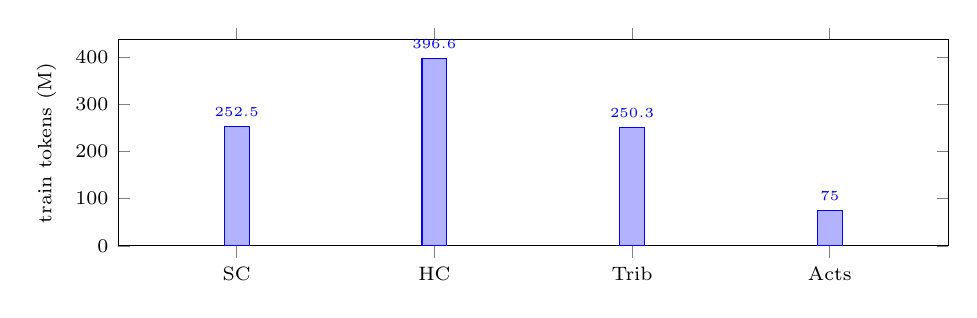
\begin{tikzpicture}
\begin{axis}[ybar, width=\linewidth, height=4.2cm, bar width=9pt, ymin=0,
  symbolic x coords={SC,HC,Trib,Acts}, xtick=data, ylabel={train tokens (M)},
  nodes near coords, every node near coord/.append style={font=\tiny},
  tick label style={font=\scriptsize}, label style={font=\scriptsize}, enlarge x limits=0.2]
\addplot coordinates {(SC,252.5) (HC,396.6) (Trib,250.3) (Acts,75.0)};
\end{axis}
\end{tikzpicture}
\caption{Phase 1 tokens per source.}
\end{subfigure}\hfill
\begin{subfigure}[t]{0.62\textwidth}
\centering
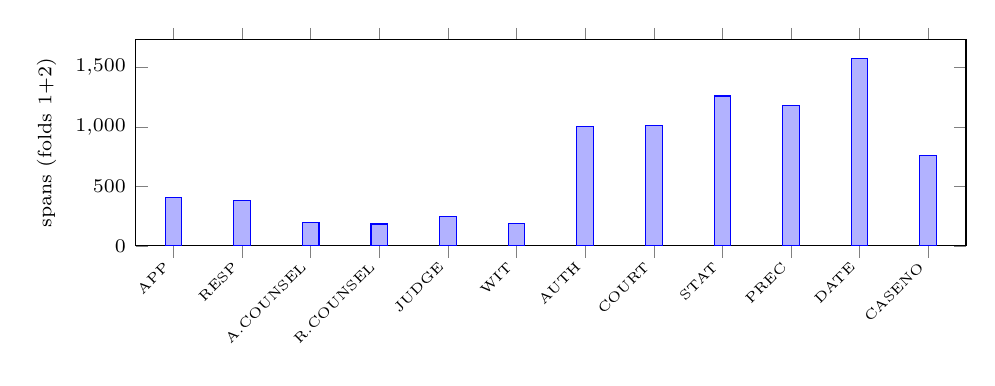
\begin{tikzpicture}
\begin{axis}[ybar, width=\linewidth, height=4.2cm, bar width=6pt, ymin=0,
  symbolic x coords={APP,RESP,A.COUNSEL,R.COUNSEL,JUDGE,WIT,AUTH,COURT,STAT,PREC,DATE,CASENO},
  xtick=data, x tick label style={rotate=45, anchor=east, font=\tiny}, ylabel={spans (folds 1+2)},
  tick label style={font=\scriptsize}, label style={font=\scriptsize}, enlarge x limits=0.05]
\addplot coordinates {(APP,407) (RESP,381) (A.COUNSEL,195) (R.COUNSEL,184) (JUDGE,245) (WIT,187) (AUTH,1003) (COURT,1013) (STAT,1260) (PREC,1183) (DATE,1575) (CASENO,760)};
\end{axis}
\end{tikzpicture}
\caption{Phase 2 entity spans per label.}
\end{subfigure}
\caption{Corpus statistics computed by our data-loading code.}
\label{fig:data}
\end{figure}

\begin{table}[H]
\centering
\footnotesize
\caption{Adaptation methods implemented ($\circ$) and used in at least one submitted run ($\bullet$) per phase. The Phase-5 KD submission was never evaluated by Codabench.}
\label{tab:methods}
\setlength{\tabcolsep}{3pt}
\begin{adjustbox}{max width=\textwidth}\begin{tabular}{c c c c c c c c c c c c c}
\toprule
Ph. & Full & Partial & BitFit & LoRA & rsLoRA & QLoRA & LoRMA & AdaLoRA & Adapter & IA$^3$ & Prompt & KD \\
\midrule
2 & $\bullet$ & $\circ$ & $\circ$ & $\circ$ & & & $\bullet$ & & & & & $\circ$ \\
3 & $\circ$ & & & $\circ$ & $\circ$ & & $\bullet$ & & & $\circ$ & $\circ$ & $\bullet$ \\
4 & $\circ$ & $\circ$ & $\circ$ & & & & $\bullet$ & $\circ$ & $\circ$ & & & $\bullet$ \\
5 & $\circ$ & $\circ$ & & & & $\circ$ & $\bullet$ & $\circ$ & $\circ$ & & $\circ$ & $\bullet$ \\
6 & $\circ$ & & & $\circ$ & & $\circ$ & $\bullet$ & $\circ$ & $\circ$ & & $\bullet$ & $\circ$ \\
7 & $\circ$ & $\circ$ & & & & $\circ$ & $\bullet$ & & & $\circ$ & $\circ$ & $\circ$ \\
\bottomrule
\end{tabular}\end{adjustbox}
\end{table}

\begin{figure}[H]
\centering
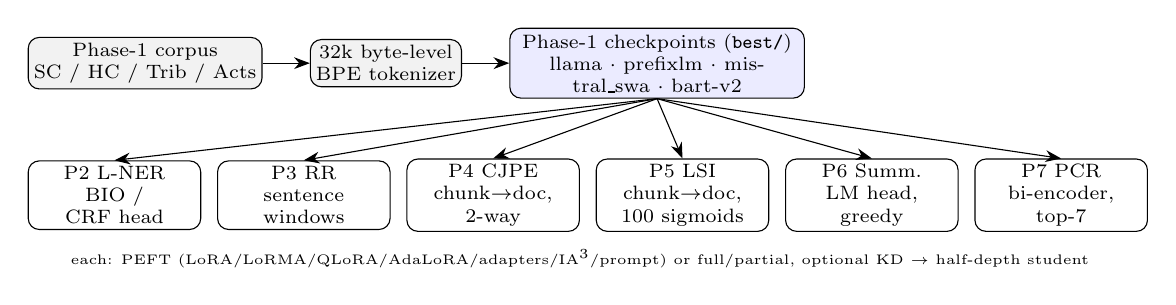
\begin{tikzpicture}[font=\scriptsize, node distance=3mm,
  box/.style={draw, rounded corners, align=center, minimum height=6mm, inner sep=2pt},
  arr/.style={-{Stealth[length=2mm]}}]
\node[box, fill=gray!10] (corpus) {Phase-1 corpus\\SC / HC / Trib / Acts};
\node[box, right=6mm of corpus, fill=gray!10] (tok) {32k byte-level\\BPE tokenizer};
\node[box, right=6mm of tok, fill=blue!8, text width=3.6cm] (p1) {Phase-1 checkpoints (\tsc{best/})\\llama $\cdot$ prefixlm $\cdot$ mistral\_swa $\cdot$ bart-v2};
\draw[arr] (corpus) -- (tok); \draw[arr] (tok) -- (p1);
\node[box, below=9mm of corpus.south west, anchor=north west, text width=2.05cm] (p2) {P2 L-NER\\BIO / CRF head};
\node[box, right=2mm of p2, text width=2.05cm] (p3) {P3 RR\\sentence windows};
\node[box, right=2mm of p3, text width=2.05cm] (p4) {P4 CJPE\\chunk$\rightarrow$doc, 2-way};
\node[box, right=2mm of p4, text width=2.05cm] (p5) {P5 LSI\\chunk$\rightarrow$doc, 100 sigmoids};
\node[box, right=2mm of p5, text width=2.05cm] (p6) {P6 Summ.\\LM head, greedy};
\node[box, right=2mm of p6, text width=2.05cm] (p7) {P7 PCR\\bi-encoder, top-7};
\foreach \n in {p2,p3,p4,p5,p6,p7} \draw[arr] (p1.south) -- (\n.north);
\node[below=1mm of p4.south east, anchor=north, font=\tiny] {each: PEFT (LoRA/LoRMA/QLoRA/AdaLoRA/adapters/IA$^3$/prompt) or full/partial, optional KD $\rightarrow$ half-depth student};
\end{tikzpicture}
\caption{System overview: one tokenizer, four pretrained backbones and six separately fine-tuned task descendants.}
\label{fig:system}
\end{figure}

\end{document}
